\section{Theoretische Grundlagen}
\label{sec:theoretische_grundlagen}
Atome können in verschiedene Energieniveaus angeregt werden. Dabei werden
Elektronen aus ihrem Grundzustand in einen Zustand höherer Energie gebracht.
Die niedrigsten Niveaus werden dabei als S- und P-Schalten bezeichnet.  Das
Verhältnis der Besetzungszahlen $N_1$ und $N_2$ dieser Zustände ohne äußeres
Magnetfeld wird dabei durch die Boltzmann-Verteilung beschrieben:
\begin{equation}
\label{eq:boltzmann}
    \frac{N_2}{N_1} = \frac{g_2}{g_1}\cdot
        \mathrm{e}^\frac{W_1 - W_2}{k_\text{B}T}\,.
\end{equation}
Dabei bezeichnet $g_i$ ein jeweiliges statistisches Gewicht, $W_i$, die
jeweilige Energie, $T$ die Temperatur und $k_\text{B}$ die bekannte
Boltzmann-Konstante.

Diese Verteilung kann durch sogenanntes optisches Pumpen, worauf im Abschnitt
\ref{subsec:optisches_pumpen} näher eingegangen wird, beeinflusst werden.
Durch Einstrahlung von Licht der Wellenlänge
\begin{equation}
\label{eq:wellenlaenge}
    h\nu = W_2 - W_1
\end{equation}
können Übergänge vom niedrigeren Energieniveau $W_1$ in das höhere Niveau
$W_2$ angeregt werden. Außerdem können Elektronen spontan oder induziert in ein
niedrigeres Niveau fallen, wobei ein neues Quant der Energie
\ref{eq:wellenlaenge} abgestrahlt wird.

\subsection{Zeeman-Effekt und Hyperfeinstruktur}
\label{subsec:zeemanneffekt_und_hyperfeinstruktur}
Die Energiestruktur von Atomen ist unter anderem durch den Gesamtdrehimpuls
$\vec{L}$ und Spin $\vec{S}$ der Elektronenhülle, sowie den Kernspin $\vec{I}$
bestimmt. Dabei sind mit diesen Drehimpulsen die magnetischen Momente
\begin{align}
    \vec{\mu}_L &= -\mu_\text{B}\vec{L}\,,
        \label{eq:magn_moment_elektronen}\\
    \vec{\mu}_S &= -g_S\mu_\text{B}\vec{S}\,,
        \label{eq:magn_moment_espin}\\
    \text{und}\qquad\vec{\mu}_I &= -g_I\mu_\text{B}\vec{I}
        \label{eq:magn_moment_kernspin}
\end{align}
verknüpft, wobei $g_I$ und $g_S$ die Landé-Faktoren bezeichnen und
$\mu_\text{B}$ das Bohrsche Magneton.
Der Gesamtdrehimpuls der Elektronenhülle koppelt dabei an den Kernspin,
was zur sogenannten Hyperfeinstruktur führt.
Zusätzlich kann der gesamte Drehimpuls $\vec{F} = \vec{J} + \vec{I}$ an äußere
magnetische Felder koppeln, was zu einer weiteren Aufspaltung in $\num{2}F +
\num{1}$ Niveaus für jedes Niveau der Hyperfeinstruktur führt.
Dieser Effekt ist in Abbildung \ref{fig:aufspaltung} schematisch dargestellt.
\begin{figure}
    \centering
    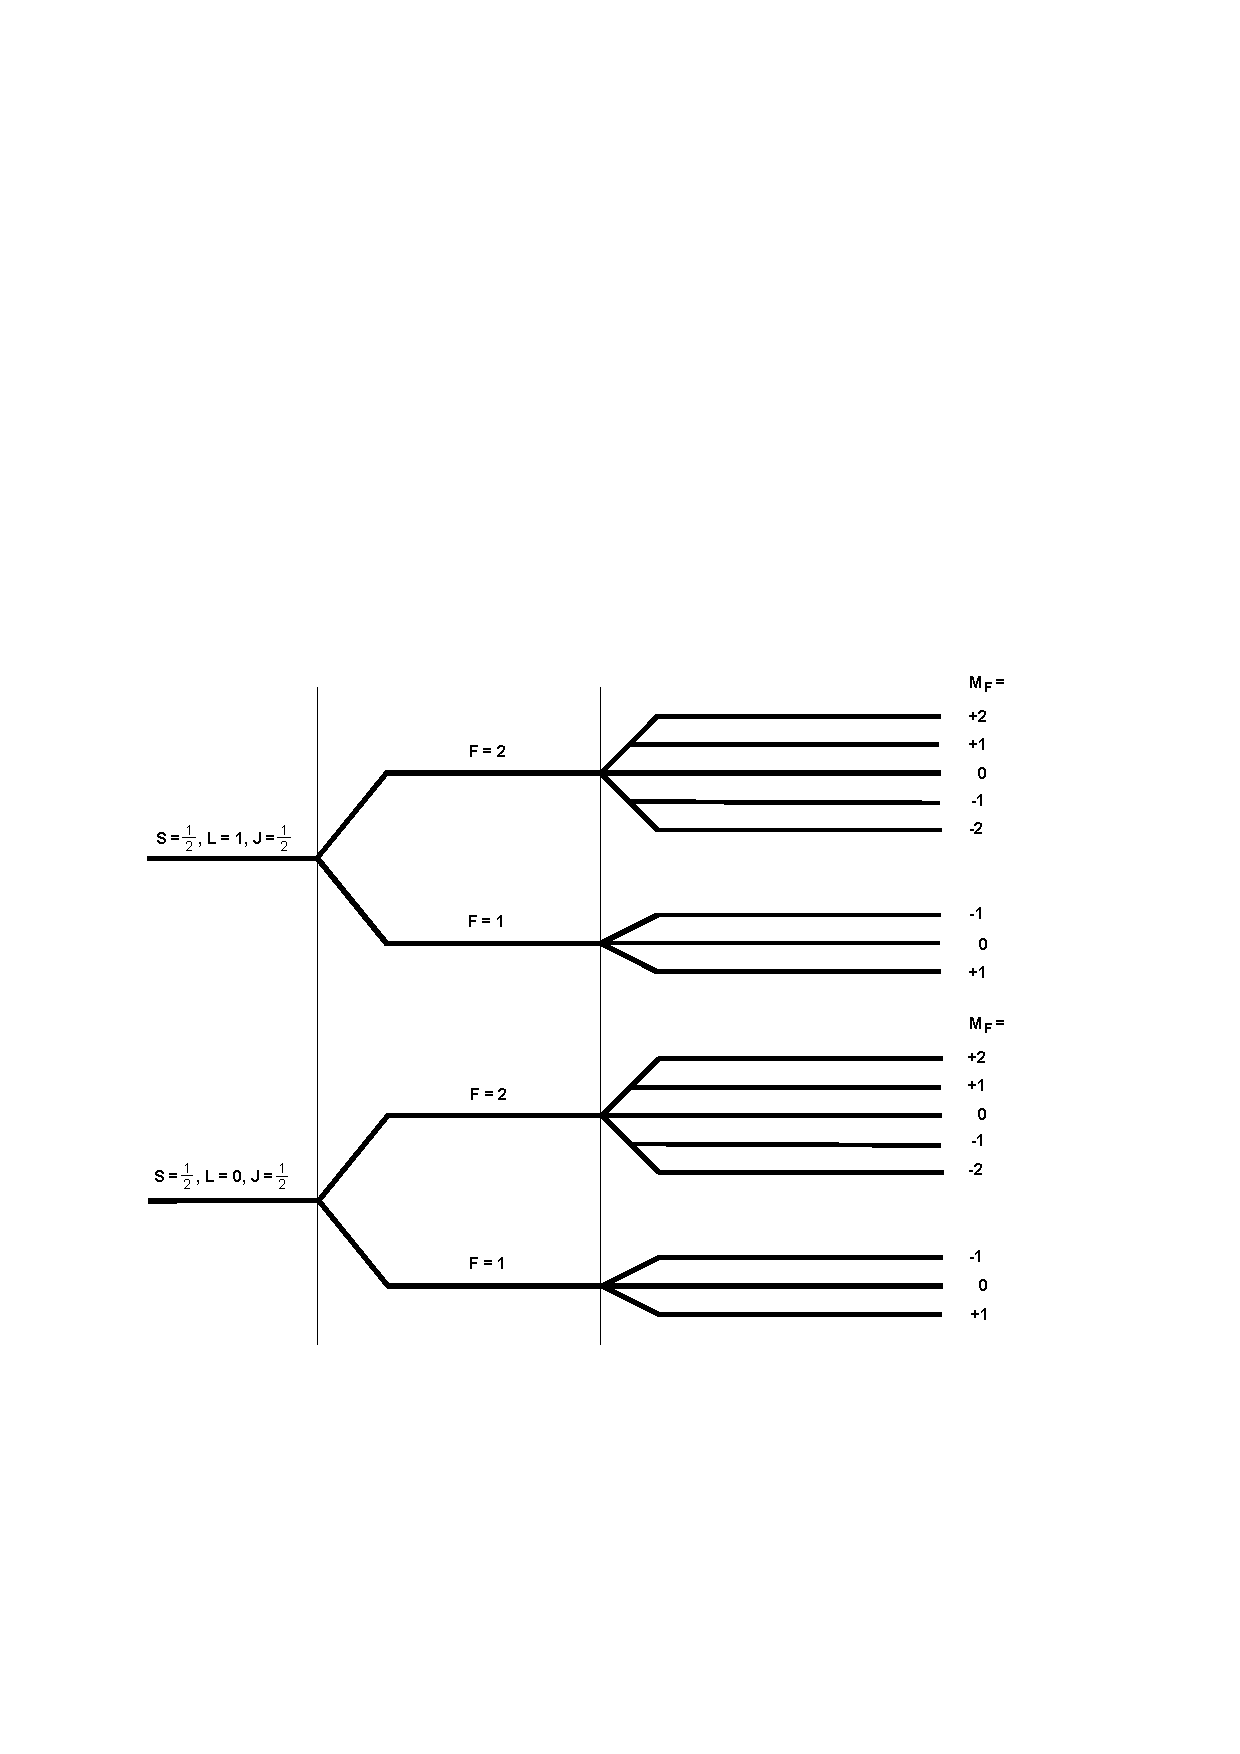
\includegraphics[width=0.8\linewidth]{img/aufspaltung.pdf}
    \caption{
        Energieaufspaltung eines Alkali-Atoms mit Kernspin $I=\sfrac{3}{2}$
        \cite{V21}.
    }
    \label{fig:aufspaltung}
\end{figure}
Die Energie benachbarter Zeeman-Niveaus unterscheidet sich dabei jeweils um
\begin{equation}
\label{eq:zeeman_energie}
    U_\text{HF} = g_F \mu_\text{B} B\,,
\end{equation}
mit dem Landé-Faktor $g_F$ und einem äußeren Magnetfeld der Feldstärke $B$.
Diese Differenz liegt üblicherweise im Bereich von einigen
\si{\micro\electronvolt} und ist damit wesentlich kleiner als andere
Energieskalen der Atomstruktur.
Aus der vektoriellen Betrachtung der magnetischen Momente und deren
Richtungsquantelung folgt für den Landé-Faktor des Atoms
\begin{equation}
\label{eq:lande_faktor}
    g_F = g_J \frac{F(F+1) + J(J+1) - I(I+1)}{2F(F+1)}\,.
\end{equation}
Da $g_S$ bekannt ist, kann ebenso $g_J$ bestimmt werden zu
\begin{equation}
\label{eq:gj}
    g_J = \frac{\num{3.0023}\cdot J(J+1)
                + \num{1.0023}\cdot\left[S(S+1) - L(L+1)\right]}
               {2J(J+1)}
          \,.
\end{equation}
Mit Hilfe des hier vorgestellten Versuchs soll der oben genannte Landé-Faktor
$g_F$ bestimmt werden.

\subsection{Optisches Pumpen}
\label{subsec:optisches_pumpen}
Übergänge zwischen zwei Energieniveaus eines Atoms können auf drei
verschiedenen Wegen von Statten gehen. Unter \emph{Absorption} eines Photons
mit einer Energie, die der Lücke zweier Niveaus entspricht kann ein Elektron in
das jeweils höhere Niveau angeregt werden.  Ein bereits angeregtes Elektron
kann spontan unter Emission eines Photons in ein niedrigeres Niveau fallen
(\emph{spontene Emission}).
Schließlich kann ein Übergang von einem höheren Niveau $W_2$ in ein niedrigeres
Niveau $W_1$ durch Einstrahlung eines Photons mit der Energie $W_2 - W_1$
stimuliert werden.  Dabei wird ein zweites Photon mit denselben Eigenschaften
des eingestrahlten Photons emittiert (\emph{induzierte Emission}).

Für diese Übergänge existieren auf Grund der Quanteneigenschaften der
Elektronen bestimmte Auswahlregeln.  Unter Einstrahlung von rechtszirkular
polarisiertem D1-Licht ($\sigma^+$-Licht) werden beispielsweise lediglich
Übergänge angeregt, für die $\Delta M = \num{+1}$ gilt.  $M$ ist dabei die
Quantenzahl der Zeeman-Aufspaltung.  Unter dieser Voraussetzung lässt sich ein
Niveau $W_1$ entleeren, wenn es keine niedrigeren Niveaus gibt, aus denen $W_1$
unter Beachtung von $\Delta M = \num{+1}$ erreicht werden kann, jedoch höhere
Niveaus mit dieser Eigenschaft existieren, die folglich befüllt werden.

Genau diese Bedingungen herrschen bei den hier untersuchten Atomen.
Durch Einstrahlung von $\sigma^+$-Licht lässt sich eine Besetzungsinversion
herstellen. Diese Übergänge werden in Abbildung \ref{fig:besetzungsinversion}
dargestellt. Der Einfachheit halber wird dabei die Hyperfeinstruktur nicht
betrachtet, der Kernspin also vernachlässigt. Eine Besetzungsinversion kann
jedoch analog zu diesem einfachen Beispiel auch mit Betrachtung des Kernspin
auftreten.
\begin{figure}
    \centering
    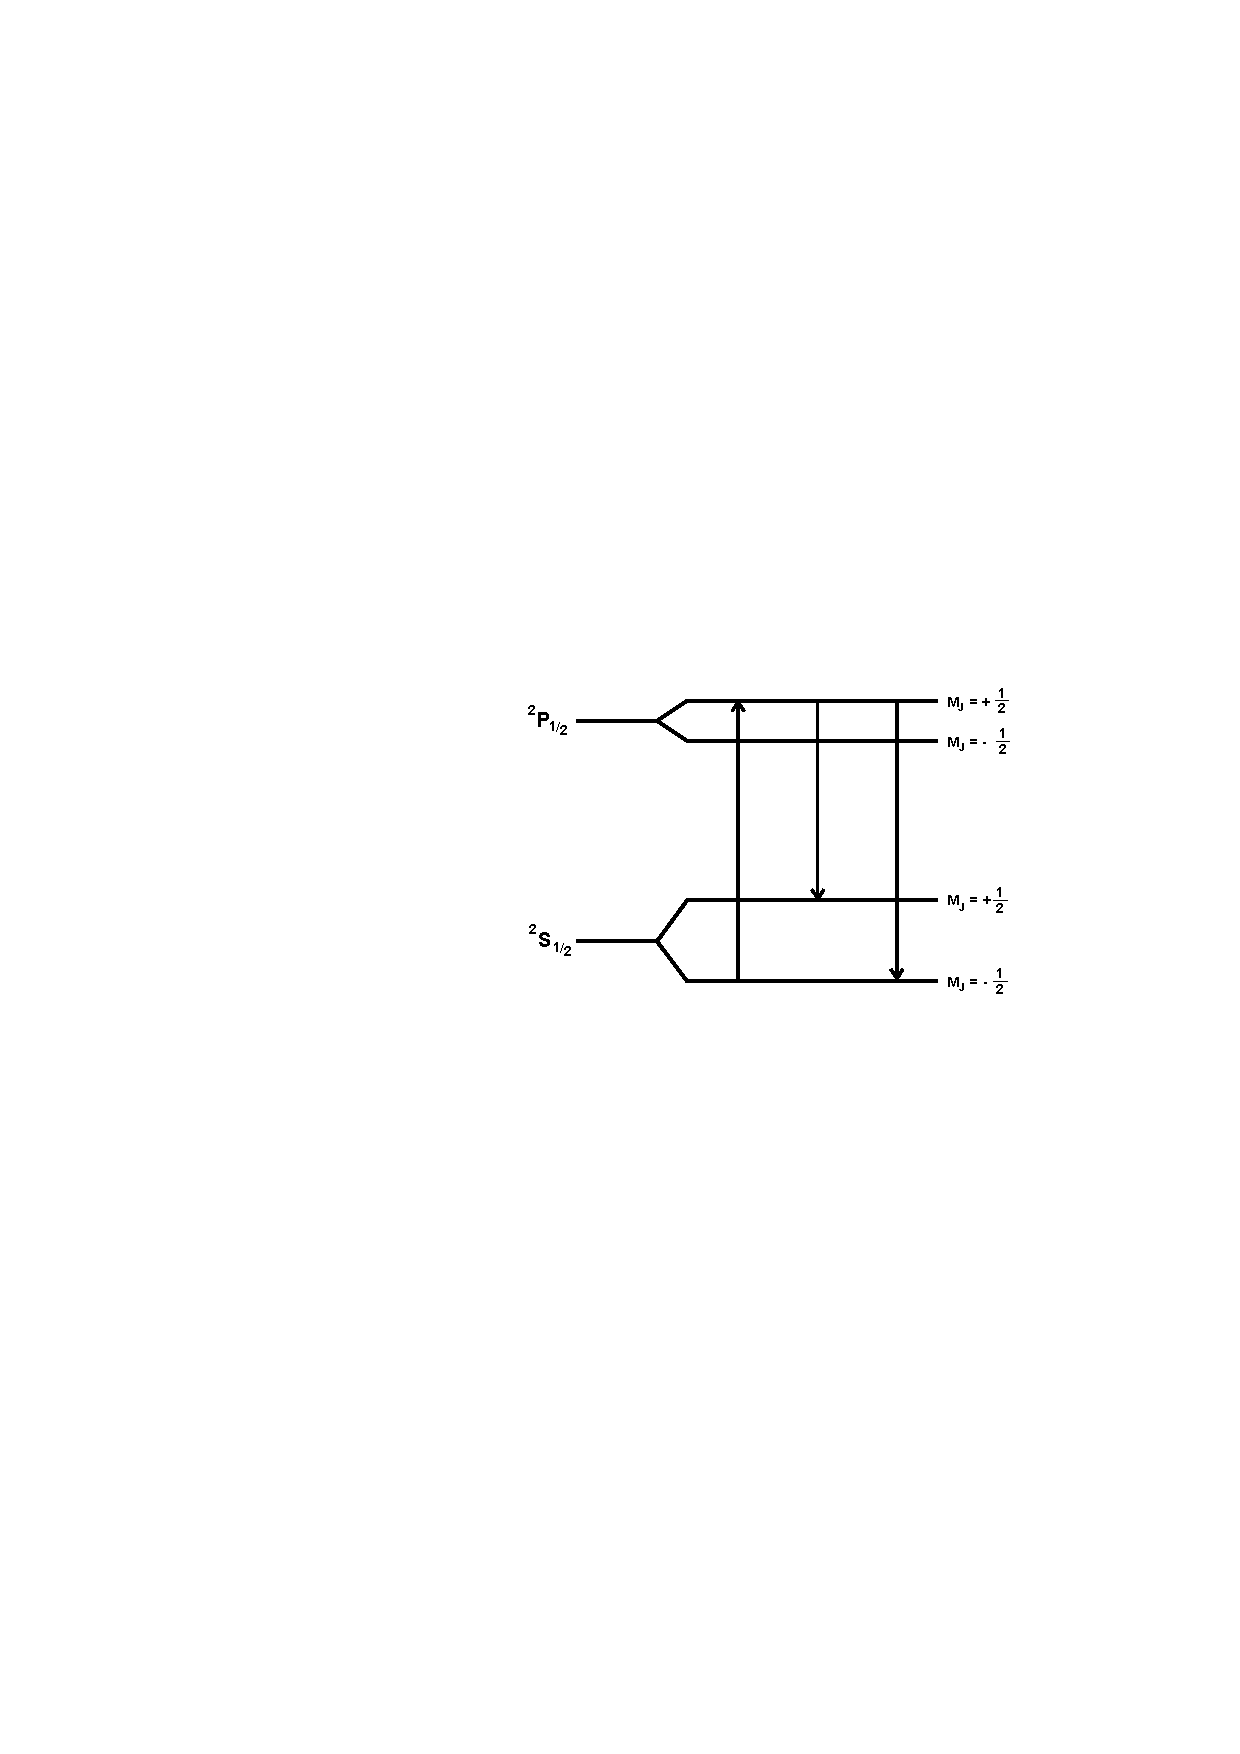
\includegraphics[width=0.7\linewidth]{img/besetzungsinversion}
    \caption{
        Energieschema eines hypothetischen Alkali-Atoms \cite{V21}. Unter
        Einstrahlung von $\sigma^+$-Licht sind lediglich die eingezeichneten
        Übergänge möglich.  Als Folge dessen lässt sich der Zustand $S,
        M_J=-\sfrac{1}{2}$ vollständig entleeren.
    }
    \label{fig:besetzungsinversion}
\end{figure}

\subsection{Messung der Zeeman-Aufspaltung}
\label{subsec:messung}
Die durch optisches Pumpen erreichte Besetzungsinversion kann durch Einkoppeln
eines elektromagnetischen Schwingfeldes rückgängig gemacht werden. Hierfür wird
die Feldstärke des Feldes variiert, bis der übervölkerte Zustand durch
induzierte Emission entleert wird. Die entsprechende Resonanzfrequenz $\nu$
genügt dann
\begin{equation}
\label{eq:resonanz}
    h\nu = g_J \mu_B B_\text{m} \Delta M_J\,,
\end{equation}
wobei $B_\text{m}$ die Magnetfeldstärke des eingestrahlten Feldes bezeichnet.

Um den Effekt der Besetzungszustände zu messen, genügt es, ein Gas der zu
untersuchenden Atome in den Strahlengang von zuvor beschriebenem
$\sigma^+$-Licht zu bringen und die Intensität des transmittierten Lichtes mit
Hilfe einer Photodiode zu messen. Herrscht Besetzungsinversion, ist das Gas
transparent, da keine Photonen mehr absorbiert werden können. Unter Variation
des Magnetfeldes $B_\text{m}$ hat die Transmissionskurve dann eine Gestalt wie
in Abbildung \ref{fig:transmission} dargestellt.
Wenn kein Feld vorhanden ist, wird das Licht absorbiert, weil es keine
Zeeman-Aufspaltung gibt. Dadurch wird das Gasgemisch undurchlässig.
Dasselbe gilt für die Situation, in welcher die Besetzungsinversion teilweise
durch induzierte Emission aufgehoben wird -- auch hier wird ein Teil des
eingestrahlten Lichtes absorbiert und die Transparenz nimmt ab.
\begin{figure}
    \centering
    \includegraphics[width=0.7\linewidth]{build/plots/transmission.pdf}
    \caption{
        Transmissionskurve in Abhängigkeit der Magnetfeldstärke $B_\text{m}$.
        Im Bereich des Nullfeldes und bei induzierter Emission (Bedingung
        \ref{eq:resonanz} ist erfüllt) verschwindet die Transmission, weil
        Absorption möglich ist.
    }
    \label{fig:transmission}
\end{figure}

\subsection{Quadratischer Zeeman-Effekt}
\label{subsec:quadratischer_zeeman-effekt}
Der in Abschnitt \ref{subsec:zeemanneffekt_und_hyperfeinstruktur}
aufgeführte Energieunterschied $U_\text{HF}$ benachbarter Zeeman-Niveaus
(\ref{eq:zeeman_energie}) gilt nur näherungsweise für kleine Magnetfeldstärken
$B$. Unter Beachtung höherer Terme der Ordnung $B^2$ erhält man den sogenannten
quadratischen Zeeman-Effekt in der Gestalt
\begin{equation}
\label{eq:quadratischer_zeeman}
    U_\text{HF} = g_F \mu_B B
        + (g_F\mu_B B)^2 \frac{1 - 2M_F}{\Delta E_\text{Hy}} - \dots\,.
\end{equation}
Hierin entspricht $\Delta E_\text{Hy}$ den Energieunterschieden benachbarter
Hyperfeinstrukturniveaus. Durch diesen Effekt werden die Energien der
Zeeman-Übergänge bei Vorliegen einer Hyperfeinstruktur leicht verschoben.

\section{Versuchsaufbau}
\label{sec:versuchsaufbau}
Für die Aufnahme der zuvor erwähnten Transmissionskurve wird der in Abbildung
\ref{fig:aufbau} schematisch dargestellte Versuchsaufbau genutzt. Das
untersuchte Gas befindet sich in einem abgeschlossenen, transparenten Gefäß,
umgeben von drei Paaren von Helmholtz-Spulen. Zwei der Spulenpaare dienen zum
Ausgleich zweier Komponenten des Erdmagnetfeldes. Das dritte Paar ermöglicht ein
Durchstimmen des effektiven Magnetfeldes, wodurch die Transmissionskurve
aufgenommen werden kann.
Eine weitere Magnetfeldspule, die mit einem Hochfrequenzsignal betrieben wird,
erzeugt Elektromagnetische Schwingfeld zur induzierten Emission.

Vor und hinter dem Gasgefäß sind optische Schienen angebracht, auf denen eine
Spektrallampe als Lichtquelle, Sammellinsen zur Strahlführung, sowie D1-Filter,
Linear-Polarisator und $\sfrac{\lambda}{4}$-Platte zur Erzeugung von
$\sigma^+$-Licht und schließlich eine Photodiode befestigt sind.

Der gesamte Aufbau kann zudem rotiert werden, um eine grobe Ausrichtung am
Erdmagnetfeld zu ermöglichen. Die horizontal ausgerichteten Helmholtz-Spulen
ermöglichen dann durch Messung eines Offset-Magnetfeldes die Bestimmung der
Feldstärke des horizontalen Erdmagnetfeldes.
\begin{figure}
    \centering
    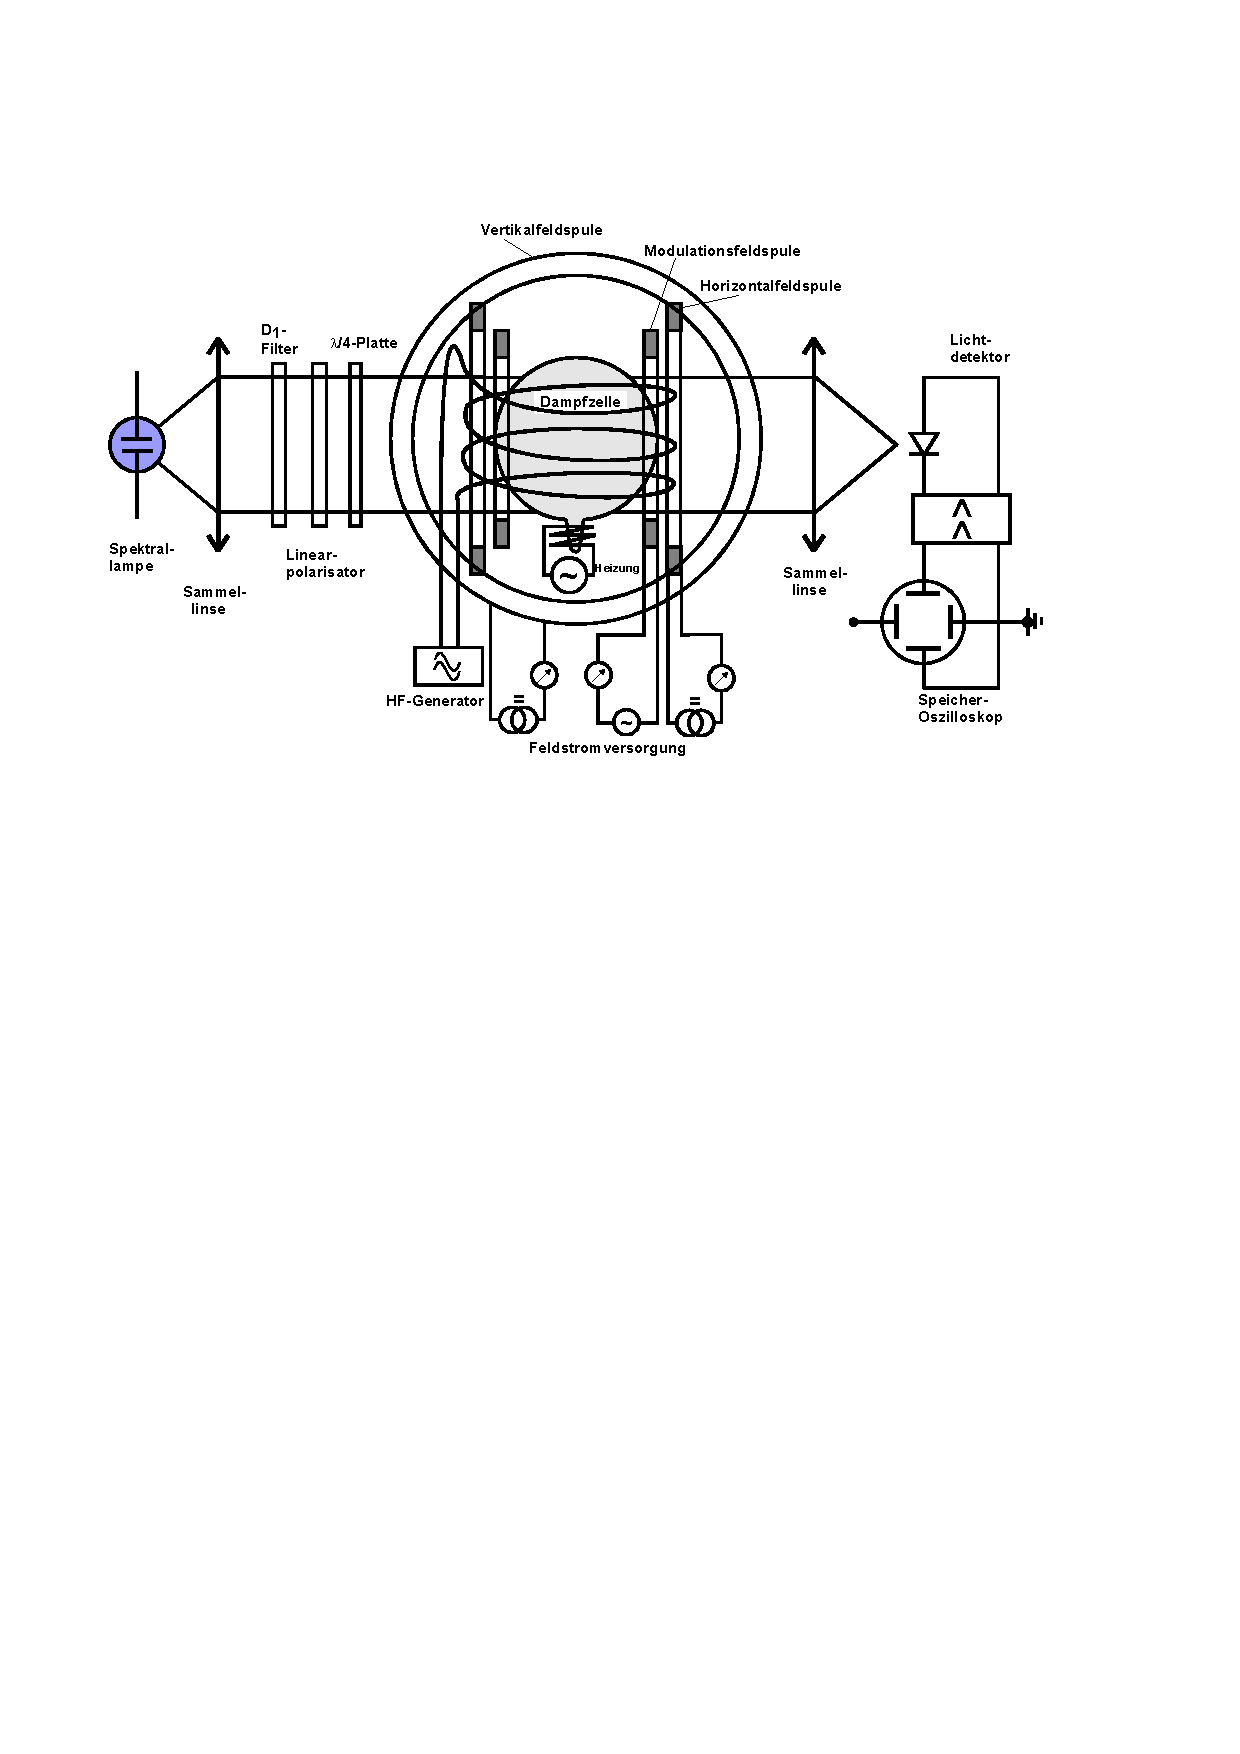
\includegraphics[width=0.9\linewidth]{img/aufbau}
    \caption{
        Schematische Darstellung des Versuchsaufbaus \cite{V21}. Auf die
        einzelnen Komponenten wird in Abschnitt \ref{sec:versuchsaufbau}
        eingegangen.
    }
    \label{fig:aufbau}
\end{figure}
